
\chapter{Conclusion \& Future Work}
\label{ch:conclusions}

\section{Thermodynamic Disorder of Cu and Zn in {\CZTS}}



\section{Further Development of Monte Carlo Disorder Models}



\section{Predicting the Photovoltaic Performance of Metal Sulfide Materials}\label{sulfosalts_proj}
As discussed in section \ref{sulfosalts_intro}, another component of this study is to predict the optoelectronic properties of other materials, which have currently received little or no attention for PV, to determine the likely performance of the materials for this application. The three candidate materials were: enargite ({\enargite}), stephanite ({\stephanite}) and bournonite ({\bournonite}). These materials are all classed as sulfosalt minerals and an overview of their known properties was given in section \ref{sulfosalts_intro}. The candidate PV materials were originally selected based on the possibility of ferroelectricity due to their polar space group and associated ferroelectric-photovoltaic phenomena, which could open up new possible pathways for high performance PV devices. However, currently in the study it is only the optoelectronic properties relevant for PV applications that are being studied.

One of the first key material properties for PV applications mentioned in section \ref{PV_properties} was the band gap of the material; both its magnitude relative to the solar spectrum and whether it is direct or indirect in nature. Therefore we firstly calculate the band structures of the materials and these are shown in figures \ref{enargite_band_structure}, \ref{stephanite_band_structure} and \ref{bournonite_band_structure} for enargite, stephanite and bournonite respectively.
Electronic structure calculations in this study are performed using the HSE06 functional \cite{HSE} as implemented in the FHI-aims software package \cite{aims, aims_hybrids, aims_parallel}, with the inclusion of spin-orbit interaction \cite{aims_SOC}.
Initial geometries are taken from high-quality X-ray diffraction data from the Inorganic Crystal Structure Database (ICSD)\cite{icsd} for enargite and bournonite and the resolved crystal structure from single crystal X-Ray diffraction measurements performed by Professor Mark Weller at the University of Bath on a natural sample of stephanite during a previous study. Geometry optimization of the structures are then performed allowing only the ionic positions to relax, holding the unit cell parameters constant.
An evenly spaced 4x4x4 \textit{k}-points grid centred on the $\Gamma$-point is used for the \textit{k}-space sampling of the first Brillouin zone as this was found to be sufficient for the total energies of the systems to converge to within 1 meV in our previous study. Convergence plots from this study are shown in an appendix.
Default `tight' accuracy convergence settings of the FHI-aims code were used for the basis sets and geometry relaxations were performed to obtain optimized structures using the Broyden-Fletcher-Goldfarb-Shanno (BFGS) optimization algorithm as implemented in the FHI-aims code \cite{aims} until forces on the atoms converged to within a tolerance of $10^{-3}$ eV/ $\AA$. Band structures were then plotted along the paths of high symmetry for each type of crystal structure.

\begin{figure}[h!]
  \centering
    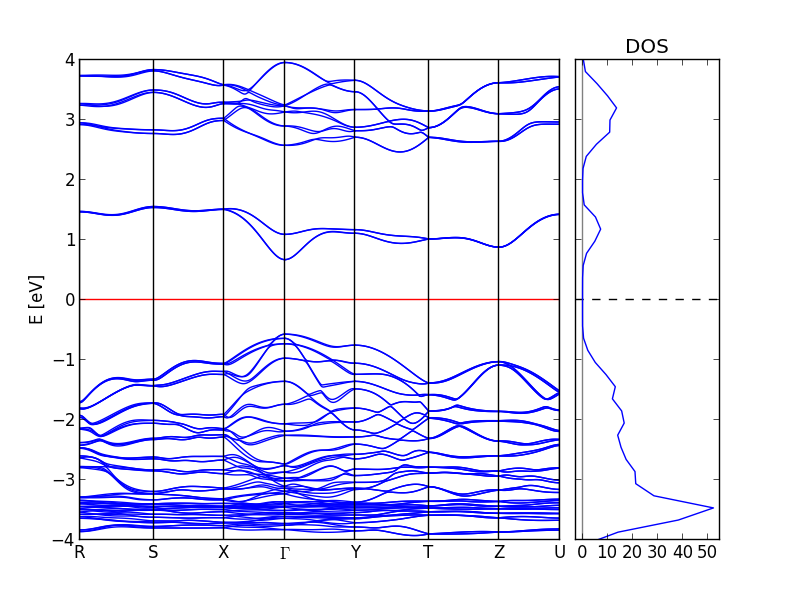
\includegraphics[width=0.9\textwidth]{figures/enargite_band_structure.png}
    \caption{}
  \label{enargite_band_structure}
\end{figure}

From our calculations, enargite has a direct band gap of 1.24 eV. This is within the range of experimental values obtained for the band gap in the literature and is also in good agreement with UV-vis measurements on a natural sample of enargite that we performed during a previous study, which gave a value of approximately 1.2 eV for the band gap. Although it should be noted that this natural sample was found to contain Sb impurities. The value we calculate is also not too far from the 1.32 eV calculated in a previous theoretical study using G$_0$W$_0$@HSE06 \cite{Zunger}.
For stephanite...
For bournonite, we calculate an indirect band gap of 1.37 eV, which is in quite good agreement with experimental values in the literature of 1.23 \cite{Dittrich1} and 1.31 \cite{bournonite} eV. However to our knowledge there are currently only calculated values for the band gap of bournonite in the literature using GGA and GGA+U methodologies. From the calculated band structure for bournonite shown in figure \ref{bournonite_band_structure}, it appears that the material could exhibit conduction band spin splitting as a consequence of spin-orbit coupling. This is often referred to as Rashba splitting. The long carrier lifetime and diffusion length observed in organometal halide perovskite solar cells has been postulated to be linked to Rashba splitting in the band structure of these materials \cite{Rashba_MAPI}. In this work the authors suggest that the rate of electron-hole recombination could be reduced due to the spin-forbidden transition, thereby resulting in enhanced carrier lifetimes.
Therefore, although the band gap we predict for bournonite is slightly indirect, it could be possible that this property could be beneficial for PV applications. The next step in investigating the optoelectronic properties of bournonite is to determine if the observed band splitting is in fact Rashba splitting. So firstly the band structure will be re-calculated with spin-orbit interaction omitted to see if the splitting is caused by spin-orbit coupling.

\begin{figure}[h!]
  \centering
    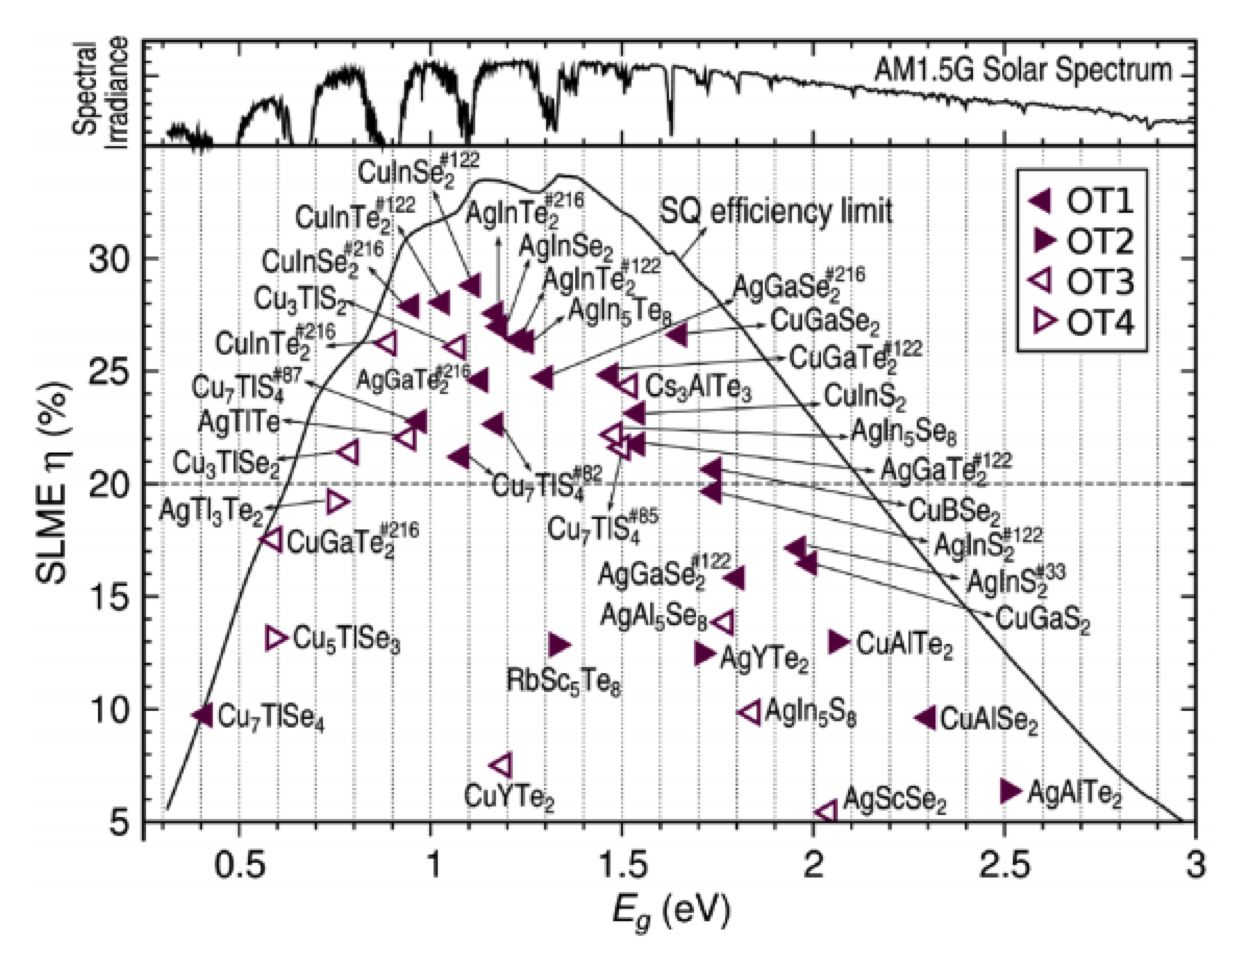
\includegraphics[width=0.9\textwidth]{figures/SLME.png}
    \caption{Spectroscopic limited maximum efficiency (SLME), $\eta$, versus the minimum band gap, E$_g$, for I-II-VI chalcopyrite materials of thickness L= 0.5 $\mu$m (triangles). The Shockley-Queisser (SQ) efficiency limit is shown by the line. Figure taken from reference \citenum{SLME}.}
  \label{SLME}
\end{figure}

However, it has been suggested that the Shockley-Queisser (SQ) theoretical efficiency limit of a solar cell based on the value of direct band gap is not a sufficient screening criteria for candidate PV materials \cite{SLME}. The authors instead suggest an alternative metric called the `spectroscopic limited maximum efficiency' (SLME), which takes into account the band gap, the shape of the optical absorption spectra and the material-dependent non-radiative recombination losses. In the same work the author's show that from their metric many materials have a maximum efficiency limit less than that predicted by SQ, this is illustrated in figure \ref{SLME}. Interestingly, the authors also find that some materials with similar band gaps (and therefore would have similar SQ limits) have very different theoretical limits from their metric. Therefore a more thorough evaluation of the potential of the candidate materials for applications in PV could be achieved by extending our investigation to encompass the SLME metric.



\section{Formation Energy of Sulfur Vacancies in Metal Sulfides}\label{Vs_proj}
CZTS work so far (neutral defect) and future work of CZTS charge corrections and sulfosalt Vs calcs - motivation is volatility of sulfur and particular synthesis methods makes this defect quite likely?\\

As discussed in section \ref{defects_in_PV}, defects in a solar absorber material can heavily impact on the performance of a photovoltaic device composed of that material. We performed calculations of the formation energy of the charge neutral Cu-on-Zn and Zn-on-Cu anti-site defect pair, [$Cu_{Zn}^- + Zn_{Cu}^+$], in order to parameterize our Monte Carlo simulations of thermodynamic Cu-Zn disorder, which was discussed in section \ref{MC_DFT}. We have also begun calculations of the formation energy of a sulfur vacancy in { \CZTS }. This defect can however take on three different charge states: $V_{S}^{0}$, $V_{S}^{+1}$ and $V_{S}^{+2}$, where electron occupancy varies from two to one to none respectively. We will then go on to calculate the formation energy as a function of the sulfur chemical potential to determine which charge state has the minimum formation energy at typical annealing conditions of { \CZTS }, in terms of temperature and pressure. Special correction techniques must be applied when performing periodic calculations to simulate a bulk system with a finite unit cell when the unit cell possesses a net charge. \\

\begin{figure}[h!]
  \centering
    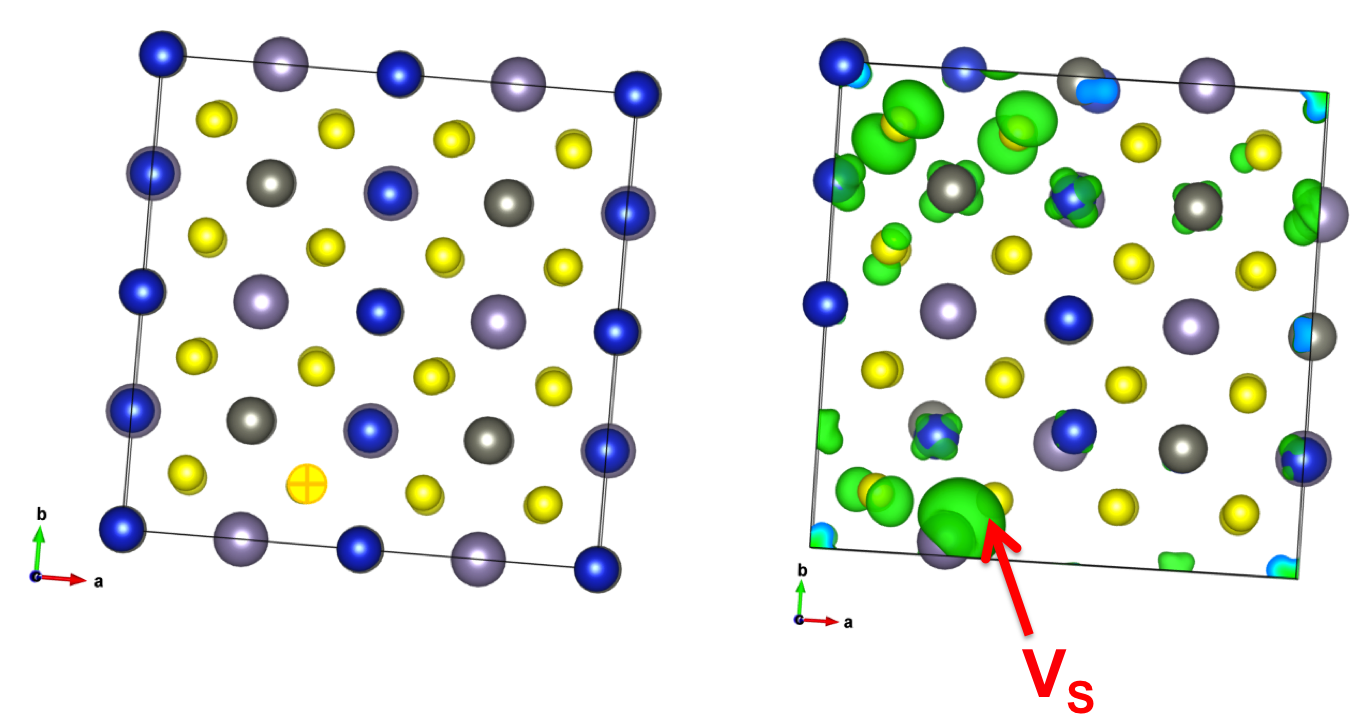
\includegraphics[width=0.9\textwidth]{figures/V_S-neutral-PARCHG.png}
    \caption{Perfect {\CZTS } supercell with S anion removed to form a sulfur vacancy (V$_S$) indicated by a crosshair (left) and the calculated partial charge density of two excess electrons present for the charge neutral V$_S$ (right).}
  \label{V_S-neutral-PARCHG}
\end{figure}

We firstly investigate the formation energy of charge neutral sulfur vacancies (V$_{S}^{0}$) as a function of the sulfur chemical potential, which itself is a function of temperature and pressure. We therefore can assess the formation energy of the vacancy under typical annealing conditions. Work from Scragg et al showed that annealing out Cu and Zn disorder can be a very time consuming process, therefore for most practical purposes some disorder will be `frozen in' after annealing. Typical annealing conditions for { \CZTS } are at ?? K and it has been shown that lower pressures are more optimal for the sulfide (whereas higher pressures are better for the selenide) **cite Adam?**. This is due to the allotropes of S?\\
On -going calculations are being performed for the charged sulfur vacancies (V$_{S}^{+1}$ and V$_{S}^{+2}$) so that the minimum energy defect, accounting for all possible charge states, across the temperature and pressure range can be determined.





\section{Intrinsic Band Gap Broadening in {\CZTS}}\label{Eg_broadening_proj}
In section \ref{PV_properties}, both effective mass and dielectric function were discussed for the insight these properties can provide for the likely PV performance of a material due to the impact these properties can have on the mobility of charge carriers in that material. However these are certainly not the only features of a real material at finite temperatures that need to be considered to understand carrier mobility in a material. 
Even in a perfect crystal, atoms are involved in some sort of thermal motion about their idealized equilibrium positions. The simplest model to describe this motion is the Einstein model where each atom vibrates independently and as a simple harmonic oscillator in the potential well created by the force fields of its neighbouring atoms. The field can never be precisely a quadratic well with spherical symmetry, but on average the approximation is reasonable, especially when only a very crude picture of thermal vibrations is sufficient or at fairly high temperatures, when the assumption that atoms vibrate independently of each other is more justified \cite{Ziman_solids}. In this model, the oscillations of the atoms can be expressed in terms of normal modes as they are independent of each other. Energies of these normal modes are then quantised, where a quantum of lattice vibration is referred to as a phonon \cite{fund_semi}.

For a given crystal structure, there are 3N phonon modes, three of which are lower-energy acoustic branches and the rest are optical curves and where N is the number of atoms in the primitive unit cell. In the case of {\CZTS}, there are therefore 24 phonon modes. Calculated phonon dispersion curves for kesterite-structured {\CZTS} are shown in figure \ref{CZTS_phonons}.
Along directions of high symmetry these phonons can be classified as transverse or longitudinal depending on whether their displacements are perpendicular or parallel to the direction of the wavevector respectively. In a solid the long wavelength transverse acoustic (TA) phonons are shear sound waves, while the longitudinal acoustic (LA) phonons are compressional sound waves. The velocities of these sound waves are determined by shear and bulk elastic moduli respectively. As it is usually easier to shear than to compress a crystal, TA phonons typically travel with lower velocities than LA phonons.  
The atomic displacements from long wavelength acoustic phonons can correspond to a deformation of the crystal, this is referred to as deformation potential theorem. Such deformations will change the electronic energies at different points in the Brillouin zone. LA phonons always produce a change in the volume of the crystal, which affects all energy bands \cite{fund_semi}.

\begin{figure}[h!]
  \centering
    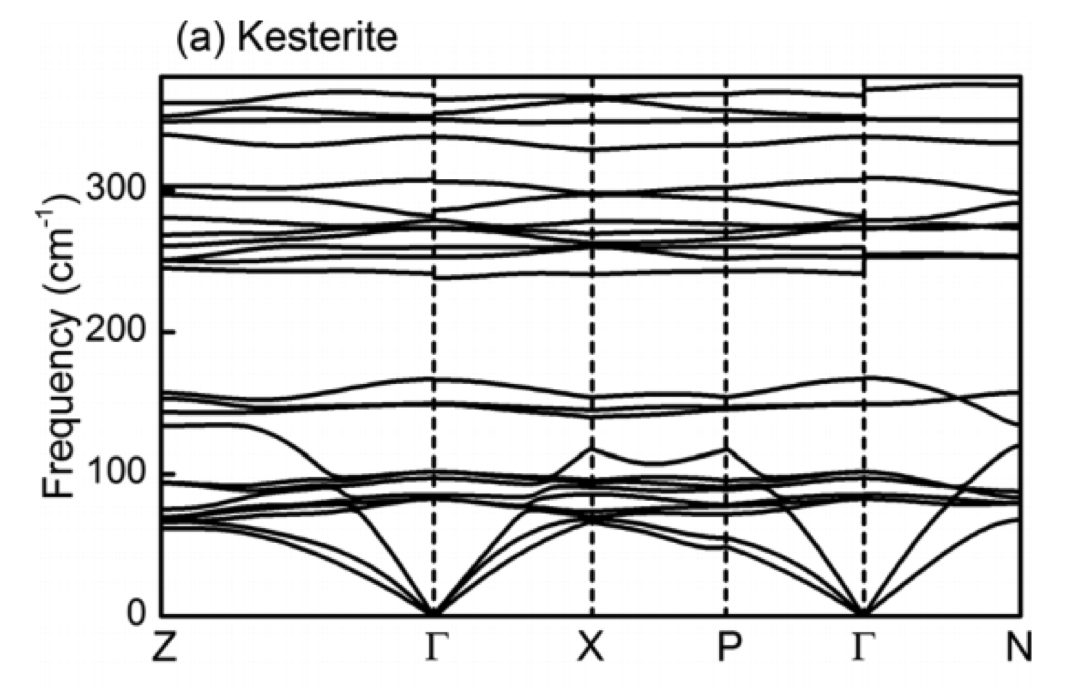
\includegraphics[width=0.7\textwidth]{figures/CZTS_phonons.png}
    \caption{Phonon dispersion curves of {\CZTS}.  Figure taken from \citenum{CZTS_phonons}.}
  \label{CZTS_phonons}
\end{figure}

The interaction of charge carriers with phonons, often referred to as electron-phonon coupling, sets a fundamental limit on the mobility of charge carriers in a material in the absence of extrinsic scattering due to defects, impurities or interfaces \cite{fund_semi, MAPI_Eg_broadening}. 
Thermal vibrations of the lattice atoms gives rise to a perturbation of the band edge \cite{thin_film_Boer}, although the interaction of charge carriers with phonons is currently still a subject of much debate \cite{MAPI_Eg_broadening16, MAPI_Eg_broadening17, MAPI_Eg_broadening}.
Of all the various possible contributions to intrinsic band gap broadening from electron-phonon coupling, there is currently no clear picture of which mechanisms are active or the most dominant in determining the carrier mobility in a material \cite{MAPI_Eg_broadening}, however it could be argued that lowest energy phonon modes are likely to make the biggest contribution. A number of studies on non-polar inorganic semiconductors have examined the temperature dependence of the charge-carrier mobility \cite{MAPI_Eg_broadening21, MAPI_Eg_broadening22, MAPI_Eg_broadening23, MAPI_Eg_broadening24}, where the carrier mobility, $\mu$, was found to scale with $T^m$ where m has a value between -1.4 and -1.6. From theory, it is known that deformation potential scattering with acoustic phonons results in $\mu \propto T^{-\frac{3}{2}}$. Therefore several works in the literature suggest that electron-phonon coupling at room temperature is dominated by acoustic phonons \cite{MAPI_Eg_broadening16, MAPI_Eg_broadening17, MAPI_Eg_broadening24}. Looking again at figure \ref{CZTS_phonons}, the acoustic modes are the three that tend to zero at the gamma point.

In on-going work, we aim to determine if the effect of the thermal motion of ions in perfect CZTS crystals could fundamentally limit carrier mobility and device performance. To do this, we have first computed the effect of volume on the band gap (the deformation potential) and have also calculated the elastic constant of bulk CZTS. So far, for CZTS we find that the band gap decreases as a result of lattice dilation, which is a trend observed in most typical semiconductors such as Si, Ge and GaAs \cite{MAPI_Eg_broadening}. This effect can be understood as a weakening of the bonds as ions are pulled apart and decreasing the separation of filled and empty states. For the next stage of this investigation, the elastic constant will be used to determine the magnitude of volume changes expected from thermal motion as a function of temperature. The deformation potential will then be used to determine the extent of band gap broadening expected to be caused by such changes in volume with temperature.
